\documentclass[a3paper]{article}
\usepackage[margin=.25in]{geometry}
\usepackage[sets,operators,adversary,advantage,probability]{cryptocode}
\usepackage{tikz}
\usepackage{amsmath}
\usepackage{amsthm}
\usepackage{hyperref}
\newcommand{\pcas}{~\highlightkeyword{as}}
\newtheorem{theorem}{Theorem}
\newtheorem{claim}{Claim}
\theoremstyle{definition}
\newtheorem{definition}{Definition}
\newcommand\lit[1]{\ensuremath{\mathtt{#1}}}
\renewcommand\O[1]{\ensuremath{\mathsf{#1}}}
\newcommand{\M}[1]{\ensuremath{\text{\texttt{#1}}}}
\newcommand{\n}[1]{\ensuremath{\mathit{#1}}}
\tikzstyle{package} = [inner sep=1pt,align=center,rounded corners,draw,minimum width=2cm,minimum height=1cm,font=\small]
\tikzstyle{onarrow} = [inner sep=1pt,font=\scriptsize,anchor=west,at start,align=left,fill=white]
\title{Theorem: freexor}
\begin{document}
\maketitle
\tableofcontents
\clearpage
\section{Games}
\begin{minipage}{.245\textwidth}
\subsection*{\hyperref[section:game:GLINRKKDM0]{GLINRKKDM0 Game}}
\scalebox{0.66}{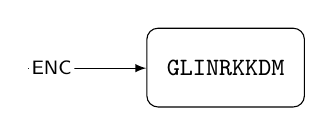
\begin{tikzpicture}
\node[anchor=south west,align=center,package,minimum height=1cm,fill=white] (node0) at (3.5,0.5) {\M{GLINRKKDM}};\draw[-latex,rounded corners] (2,1) -- node[onarrow] {\O{ENC}} (3.5,1);
\end{tikzpicture}
}
\end{minipage}
\begin{minipage}{.245\textwidth}
\subsection*{\hyperref[section:game:GLINRKKDM1]{GLINRKKDM1 Game}}
\scalebox{0.66}{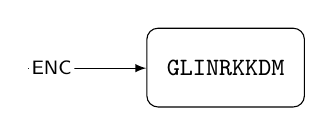
\begin{tikzpicture}
\node[anchor=south west,align=center,package,minimum height=1cm,fill=white] (node0) at (3.5,0.5) {\M{GLINRKKDM}};\draw[-latex,rounded corners] (2,1) -- node[onarrow] {\O{ENC}} (3.5,1);
\end{tikzpicture}
}
\end{minipage}
\begin{minipage}{.245\textwidth}
\subsection*{\hyperref[section:game:RcompGLINRKKDM0]{RcompGLINRKKDM0 Game}}
\scalebox{0.66}{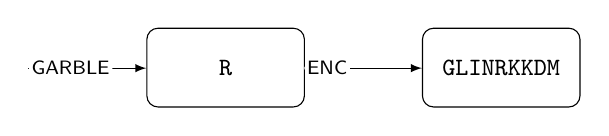
\begin{tikzpicture}
\node[anchor=south west,align=center,package,minimum height=1cm,fill=white] (node0) at (7,0.5) {\M{GLINRKKDM}};\node[anchor=south west,align=center,package,minimum height=1cm,fill=white] (node1) at (3.5,0.5) {\M{R}};\draw[-latex,rounded corners]
    (5.5,1) -- node[onarrow] {\O{ENC}} (7,1);
\draw[-latex,rounded corners] (2,1) -- node[onarrow] {\O{GARBLE}} (3.5,1);
\end{tikzpicture}
}
\end{minipage}
\begin{minipage}{.245\textwidth}
\subsection*{\hyperref[section:game:RcompGLINRKKDM1]{RcompGLINRKKDM1 Game}}
\scalebox{0.66}{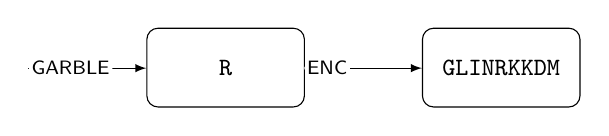
\begin{tikzpicture}
\node[anchor=south west,align=center,package,minimum height=1cm,fill=white] (node0) at (7,0.5) {\M{GLINRKKDM}};\node[anchor=south west,align=center,package,minimum height=1cm,fill=white] (node1) at (3.5,0.5) {\M{R}};\draw[-latex,rounded corners]
    (5.5,1) -- node[onarrow] {\O{ENC}} (7,1);
\draw[-latex,rounded corners] (2,1) -- node[onarrow] {\O{GARBLE}} (3.5,1);
\end{tikzpicture}
}
\end{minipage}
\\
\begin{minipage}{.245\textwidth}
\subsection*{\hyperref[section:game:GSimFreeXORReal]{GSimFreeXORReal Game}}
\scalebox{0.66}{\input{CompositionGraph_GSimFreeXORReal.tex}}
\end{minipage}
\begin{minipage}{.245\textwidth}
\subsection*{\hyperref[section:game:GSimFreeXORIdeal]{GSimFreeXORIdeal Game}}
\scalebox{0.66}{\input{CompositionGraph_GSimFreeXORIdeal.tex}}
\end{minipage}
\clearpage
\subsection{GLINRKKDM0 Game}
\label{section:game:GLINRKKDM0}
\begin{center}
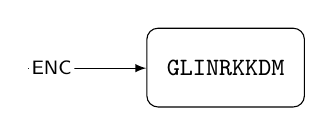
\begin{tikzpicture}
\node[anchor=south west,align=center,package,minimum height=1cm,fill=white] (node0) at (3.5,0.5) {\M{GLINRKKDM}};\draw[-latex,rounded corners] (2,1) -- node[onarrow] {\O{ENC}} (3.5,1);
\end{tikzpicture}

\end{center}
\begin{pchstack}
\begin{pcvstack}\underline{\underline{\M{GLINRKKDM}}}\\\begin{pcvstack}
\procedure{$\O{ENC}(\n{key}, \n{msg}, \n{z})$}{
\pcif \n{delta} = \bot \pcthen\\
\pcind \n{tmp} \stackrel{delta}{\sample} \bin^{\n{n}}\\
\pcind \n{delta} \gets \n{tmp}\\
 \n{r} \stackrel{2}{\sample} \bin^{\n{n}}\\
\pcif \n{b} \pcthen\\
\pcind \pcreturn \O{\n{enc}}(\O{\n{xor}^\prime}(\n{delta}, \n{key}), Expression { kind: BitsLiteral("0", Type { kind: Bits(Identifier(PackageIdentifier(Const(PackageConstIdentifier { pkg_name: "LINRKKDM", name: "n", ty: Type { kind: Integer }, game_assignment: Some(Expression { kind: Identifier(GameIdentifier(Const(GameConstIdentifier { game_name: "GLINRKKDM", name: "n", ty: Type { kind: Integer }, game_inst_name: None, theorem_name: None, inst_info: None, assigned_value: None }))) }), pkg_inst_name: Some("GLINRKKDM"), game_name: Some("GLINRKKDM"), game_inst_name: None, theorem_name: None })))) }) }, \n{r})\\
\pcelse\\
\pcind\pcif \n{z} \pcthen\\
\pcind\pcind \pcreturn \O{\n{enc}}(\O{\n{xor}^\prime}(\n{delta}, \n{key}), \O{\n{xor}^\prime}(\n{msg}, \n{delta}), \n{r})\\
\pcind\pcelse\\
\pcind\pcind \pcreturn \O{\n{enc}}(\O{\n{xor}^\prime}(\n{delta}, \n{key}), \n{msg}, \n{r})\\
}
\pcvspace
\end{pcvstack}\end{pcvstack}

\pchspace
\end{pchstack}
\clearpage
\subsection{GLINRKKDM1 Game}
\label{section:game:GLINRKKDM1}
\begin{center}
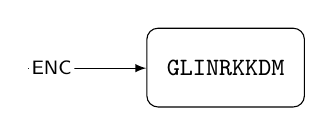
\begin{tikzpicture}
\node[anchor=south west,align=center,package,minimum height=1cm,fill=white] (node0) at (3.5,0.5) {\M{GLINRKKDM}};\draw[-latex,rounded corners] (2,1) -- node[onarrow] {\O{ENC}} (3.5,1);
\end{tikzpicture}

\end{center}
\begin{pchstack}
\begin{pcvstack}\underline{\underline{\M{GLINRKKDM}}}\\\begin{pcvstack}
\procedure{$\O{ENC}(\n{key}, \n{msg}, \n{z})$}{
\pcif \n{delta} = \bot \pcthen\\
\pcind \n{tmp} \stackrel{delta}{\sample} \bin^{\n{n}}\\
\pcind \n{delta} \gets \n{tmp}\\
 \n{r} \stackrel{2}{\sample} \bin^{\n{n}}\\
\pcif \n{b} \pcthen\\
\pcind \pcreturn \O{\n{enc}}(\O{\n{xor}^\prime}(\n{delta}, \n{key}), Expression { kind: BitsLiteral("0", Type { kind: Bits(Identifier(PackageIdentifier(Const(PackageConstIdentifier { pkg_name: "LINRKKDM", name: "n", ty: Type { kind: Integer }, game_assignment: Some(Expression { kind: Identifier(GameIdentifier(Const(GameConstIdentifier { game_name: "GLINRKKDM", name: "n", ty: Type { kind: Integer }, game_inst_name: None, theorem_name: None, inst_info: None, assigned_value: None }))) }), pkg_inst_name: Some("GLINRKKDM"), game_name: Some("GLINRKKDM"), game_inst_name: None, theorem_name: None })))) }) }, \n{r})\\
\pcelse\\
\pcind\pcif \n{z} \pcthen\\
\pcind\pcind \pcreturn \O{\n{enc}}(\O{\n{xor}^\prime}(\n{delta}, \n{key}), \O{\n{xor}^\prime}(\n{msg}, \n{delta}), \n{r})\\
\pcind\pcelse\\
\pcind\pcind \pcreturn \O{\n{enc}}(\O{\n{xor}^\prime}(\n{delta}, \n{key}), \n{msg}, \n{r})\\
}
\pcvspace
\end{pcvstack}\end{pcvstack}

\pchspace
\end{pchstack}
\clearpage
\subsection{RcompGLINRKKDM0 Game}
\label{section:game:RcompGLINRKKDM0}
\begin{center}
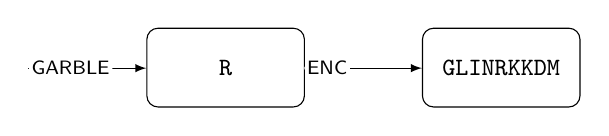
\begin{tikzpicture}
\node[anchor=south west,align=center,package,minimum height=1cm,fill=white] (node0) at (7,0.5) {\M{GLINRKKDM}};\node[anchor=south west,align=center,package,minimum height=1cm,fill=white] (node1) at (3.5,0.5) {\M{R}};\draw[-latex,rounded corners]
    (5.5,1) -- node[onarrow] {\O{ENC}} (7,1);
\draw[-latex,rounded corners] (2,1) -- node[onarrow] {\O{GARBLE}} (3.5,1);
\end{tikzpicture}

\end{center}
\begin{pchstack}
\begin{pcvstack}\underline{\underline{\M{GLINRKKDM}}}\\\begin{pcvstack}
\input{Oracle_GLINRKKDM_ENC_in_RcompGLINRKKDM_lossy.tex}\pcvspace
\end{pcvstack}\end{pcvstack}

\pchspace
\begin{pcvstack}\underline{\underline{\M{R}}}\\\begin{pcvstack}
\input{Oracle_R_GARBLE_in_RcompGLINRKKDM_lossy.tex}\pcvspace
\end{pcvstack}\end{pcvstack}

\pchspace
\end{pchstack}
\clearpage
\subsection{RcompGLINRKKDM1 Game}
\label{section:game:RcompGLINRKKDM1}
\begin{center}
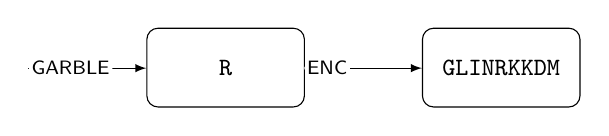
\begin{tikzpicture}
\node[anchor=south west,align=center,package,minimum height=1cm,fill=white] (node0) at (7,0.5) {\M{GLINRKKDM}};\node[anchor=south west,align=center,package,minimum height=1cm,fill=white] (node1) at (3.5,0.5) {\M{R}};\draw[-latex,rounded corners]
    (5.5,1) -- node[onarrow] {\O{ENC}} (7,1);
\draw[-latex,rounded corners] (2,1) -- node[onarrow] {\O{GARBLE}} (3.5,1);
\end{tikzpicture}

\end{center}
\begin{pchstack}
\begin{pcvstack}\underline{\underline{\M{GLINRKKDM}}}\\\begin{pcvstack}
\input{Oracle_GLINRKKDM_ENC_in_RcompGLINRKKDM_lossy.tex}\pcvspace
\end{pcvstack}\end{pcvstack}

\pchspace
\begin{pcvstack}\underline{\underline{\M{R}}}\\\begin{pcvstack}
\input{Oracle_R_GARBLE_in_RcompGLINRKKDM_lossy.tex}\pcvspace
\end{pcvstack}\end{pcvstack}

\pchspace
\end{pchstack}
\clearpage
\subsection{GSimFreeXORReal Game}
\label{section:game:GSimFreeXORReal}
\begin{center}
\input{CompositionGraph_GSimFreeXORReal.tex}
\end{center}
\begin{pchstack}
\begin{pcvstack}\underline{\underline{\M{SimFreeXOR0}}}\\\begin{pcvstack}
\procedure{$\O{GARBLE}(\n{f}, \n{x})$}{
 \left(\n{a}, \n{b}\right) \gets \n{x}\\
 \n{delta} \stackrel{delta}{\sample} \bin^{\n{n}}\\
 \n{R}_\n{00} \stackrel{R\_00}{\sample} \bin^{\n{n}}\\
 \n{R}_\n{01} \stackrel{R\_01}{\sample} \bin^{\n{n}}\\
 \n{R}_\n{10} \stackrel{R\_10}{\sample} \bin^{\n{n}}\\
 \n{R}_\n{11} \stackrel{R\_11}{\sample} \bin^{\n{n}}\\
 \n{o} \stackrel{6}{\sample} \bin^{\n{m}}\\
 \n{oo} \stackrel{7}{\sample} \bin^{\n{n}}\\
 \n{C}^\prime \gets \left(\begin{array}{c}\pclb\left(\begin{array}{c}\n{o}, \n{o}\end{array}\right), \pclb\left(\begin{array}{c}\n{o}, \n{o}\end{array}\right), \pclb\left(\begin{array}{c}\n{o}, \n{o}\end{array}\right), \pclb\left(\begin{array}{c}\n{o}, \n{o}\end{array}\right)\end{array}\right)\\
 \n{X}^\prime \gets \left(\begin{array}{c}\n{oo}, \n{oo}\end{array}\right)\\
 \n{d} \gets \O{EmptyTable}(\O{Table}[\bin^{\n{n}} \rightarrow \O{Boolean}])\\
 \n{tempsample1} \stackrel{A\_0}{\sample} \bin^{\n{n}}\\
 \n{tempsample2} \stackrel{B\_0}{\sample} \bin^{\n{n}}\\
 \n{tempsample3} \stackrel{C\_0}{\sample} \bin^{\n{n}}\\
\pcif \left(\n{a} = \lit{false} \wedge \n{b} = \lit{false}\right) \pcthen\\
\pcind \n{c} \gets \lit{false}\\
\pcind \n{A}_\n{0} \gets \n{tempsample1}\\
\pcind \n{B}_\n{0} \gets \n{tempsample2}\\
\pcind \n{C}_\n{0} \gets \n{tempsample3}\\
\pcind \n{A}_\n{1} \gets \O{\n{xor}^\prime}(\n{A}_\n{0}, \n{delta})\\
\pcind \n{B}_\n{1} \gets \O{\n{xor}^\prime}(\n{B}_\n{0}, \n{delta})\\
\pcind \n{C}_\n{1} \gets \O{\n{xor}^\prime}(\n{C}_\n{0}, \n{delta})\\
\pcind \n{r} \stackrel{11}{\sample} \bin^{\n{n}}\\
\pcind \n{r1} \stackrel{12}{\sample} \bin^{\n{n}}\\
\pcind \n{GarbledRow0} \gets \left(\begin{array}{c}\pclb\O{\n{enc}}(\n{A}_\n{0}, \n{R}_\n{00}, \n{r}), \pclb\O{\n{enc}}(\n{B}_\n{0}, \O{\n{xor}^\prime}(\n{R}_\n{00}, \n{C}_\n{0}), \n{r1})\end{array}\right)\\
\pcind \n{r} \stackrel{13}{\sample} \bin^{\n{n}}\\
\pcind \n{r1} \stackrel{14}{\sample} \bin^{\n{n}}\\
\pcind \n{GarbledRow1} \gets \left(\begin{array}{c}\pclb\O{\n{enc}}(\n{A}_\n{0}, \n{R}_\n{01}, \n{r}), \pclb\O{\n{enc}}(\n{B}_\n{1}, \O{\n{xor}^\prime}(\n{R}_\n{01}, \n{C}_\n{0}), \n{r1})\end{array}\right)\\
\pcind \n{r} \stackrel{15}{\sample} \bin^{\n{n}}\\
\pcind \n{r1} \stackrel{16}{\sample} \bin^{\n{n}}\\
\pcind \n{GarbledRow2} \gets \left(\begin{array}{c}\pclb\O{\n{enc}}(\n{A}_\n{1}, \n{R}_\n{10}, \n{r}), \pclb\O{\n{enc}}(\n{B}_\n{0}, \O{\n{xor}^\prime}(\n{R}_\n{10}, \n{C}_\n{0}), \n{r1})\end{array}\right)\\
\pcind \n{r} \stackrel{17}{\sample} \bin^{\n{n}}\\
\pcind \n{r1} \stackrel{18}{\sample} \bin^{\n{n}}\\
\pcind \n{GarbledRow3} \gets \left(\begin{array}{c}\pclb\O{\n{enc}}(\n{A}_\n{1}, \n{R}_\n{11}, \n{r}), \pclb\O{\n{enc}}(\n{B}_\n{1}, \O{\n{xor}^\prime}(\n{R}_\n{11}, \n{C}_\n{1}), \n{r1})\end{array}\right)\\
\pcind \n{C}^\prime \gets \left(\begin{array}{c}\n{GarbledRow0}, \pclb\n{GarbledRow1}, \pclb\n{GarbledRow2}, \pclb\n{GarbledRow3}\end{array}\right)\\
\pcind \n{X}^\prime \gets \left(\begin{array}{c}\n{A}_\n{0}, \n{B}_\n{0}\end{array}\right)\\
\pcind \n{d}\left[\n{C}_\n{0}\right] \gets \n{c}\\
\pcif \left(\n{a} = \lit{false} \wedge \n{b} = \lit{true}\right) \pcthen\\
\pcind \n{c} \gets \lit{false}\\
\pcind \n{A}_\n{0} \gets \n{tempsample1}\\
\pcind \n{B}_\n{1} \gets \n{tempsample2}\\
\pcind \n{C}_\n{0} \gets \n{tempsample3}\\
\pcind \n{A}_\n{1} \gets \O{\n{xor}^\prime}(\n{A}_\n{0}, \n{delta})\\
\pcind \n{B}_\n{0} \gets \O{\n{xor}^\prime}(\n{B}_\n{1}, \n{delta})\\
\pcind \n{C}_\n{1} \gets \O{\n{xor}^\prime}(\n{C}_\n{0}, \n{delta})\\
\pcind \n{r} \stackrel{19}{\sample} \bin^{\n{n}}\\
\pcind \n{r1} \stackrel{20}{\sample} \bin^{\n{n}}\\
\pcind \n{GarbledRow1} \gets \left(\begin{array}{c}\pclb\O{\n{enc}}(\n{A}_\n{0}, \n{R}_\n{01}, \n{r}), \pclb\O{\n{enc}}(\n{B}_\n{1}, \O{\n{xor}^\prime}(\n{R}_\n{01}, \n{C}_\n{0}), \n{r1})\end{array}\right)\\
\pcind \n{r} \stackrel{21}{\sample} \bin^{\n{n}}\\
\pcind \n{r1} \stackrel{22}{\sample} \bin^{\n{n}}\\
\pcind \n{GarbledRow0} \gets \left(\begin{array}{c}\pclb\O{\n{enc}}(\n{A}_\n{0}, \n{R}_\n{00}, \n{r}), \pclb\O{\n{enc}}(\n{B}_\n{0}, \O{\n{xor}^\prime}(\n{R}_\n{00}, \n{C}_\n{0}), \n{r1})\end{array}\right)\\
\pcind \n{r} \stackrel{23}{\sample} \bin^{\n{n}}\\
\pcind \n{r1} \stackrel{24}{\sample} \bin^{\n{n}}\\
\pcind \n{GarbledRow3} \gets \left(\begin{array}{c}\pclb\O{\n{enc}}(\n{A}_\n{1}, \n{R}_\n{11}, \n{r}), \pclb\O{\n{enc}}(\n{B}_\n{1}, \O{\n{xor}^\prime}(\n{R}_\n{11}, \n{C}_\n{1}), \n{r1})\end{array}\right)\\
\pcind \n{r} \stackrel{25}{\sample} \bin^{\n{n}}\\
\pcind \n{r1} \stackrel{26}{\sample} \bin^{\n{n}}\\
\pcind \n{GarbledRow2} \gets \left(\begin{array}{c}\pclb\O{\n{enc}}(\n{A}_\n{1}, \n{R}_\n{10}, \n{r}), \pclb\O{\n{enc}}(\n{B}_\n{0}, \O{\n{xor}^\prime}(\n{R}_\n{10}, \n{C}_\n{0}), \n{r1})\end{array}\right)\\
\pcind \n{C}^\prime \gets \left(\begin{array}{c}\n{GarbledRow0}, \pclb\n{GarbledRow1}, \pclb\n{GarbledRow2}, \pclb\n{GarbledRow3}\end{array}\right)\\
\pcind \n{X}^\prime \gets \left(\begin{array}{c}\n{A}_\n{0}, \n{B}_\n{1}\end{array}\right)\\
\pcind \n{d}\left[\n{C}_\n{0}\right] \gets \n{c}\\
\pcif \left(\n{a} = \lit{true} \wedge \n{b} = \lit{false}\right) \pcthen\\
\pcind \n{c} \gets \lit{false}\\
\pcind \n{A}_\n{1} \gets \n{tempsample1}\\
\pcind \n{B}_\n{0} \gets \n{tempsample2}\\
\pcind \n{C}_\n{0} \gets \n{tempsample3}\\
\pcind \n{A}_\n{0} \gets \O{\n{xor}^\prime}(\n{A}_\n{1}, \n{delta})\\
\pcind \n{B}_\n{1} \gets \O{\n{xor}^\prime}(\n{B}_\n{0}, \n{delta})\\
\pcind \n{C}_\n{1} \gets \O{\n{xor}^\prime}(\n{C}_\n{0}, \n{delta})\\
\pcind \n{r} \stackrel{27}{\sample} \bin^{\n{n}}\\
\pcind \n{r1} \stackrel{28}{\sample} \bin^{\n{n}}\\
\pcind \n{GarbledRow2} \gets \left(\begin{array}{c}\pclb\O{\n{enc}}(\n{A}_\n{1}, \n{R}_\n{10}, \n{r}), \pclb\O{\n{enc}}(\n{B}_\n{0}, \O{\n{xor}^\prime}(\n{R}_\n{10}, \n{C}_\n{0}), \n{r1})\end{array}\right)\\
\pcind \n{r} \stackrel{29}{\sample} \bin^{\n{n}}\\
\pcind \n{r1} \stackrel{30}{\sample} \bin^{\n{n}}\\
\pcind \n{GarbledRow3} \gets \left(\begin{array}{c}\pclb\O{\n{enc}}(\n{A}_\n{1}, \n{R}_\n{11}, \n{r}), \pclb\O{\n{enc}}(\n{B}_\n{1}, \O{\n{xor}^\prime}(\n{R}_\n{11}, \n{C}_\n{1}), \n{r1})\end{array}\right)\\
\pcind \n{r} \stackrel{31}{\sample} \bin^{\n{n}}\\
\pcind \n{r1} \stackrel{32}{\sample} \bin^{\n{n}}\\
\pcind \n{GarbledRow0} \gets \left(\begin{array}{c}\pclb\O{\n{enc}}(\n{A}_\n{0}, \n{R}_\n{00}, \n{r}), \pclb\O{\n{enc}}(\n{B}_\n{0}, \O{\n{xor}^\prime}(\n{R}_\n{00}, \n{C}_\n{0}), \n{r1})\end{array}\right)\\
\pcind \n{r} \stackrel{33}{\sample} \bin^{\n{n}}\\
\pcind \n{r1} \stackrel{34}{\sample} \bin^{\n{n}}\\
\pcind \n{GarbledRow1} \gets \left(\begin{array}{c}\pclb\O{\n{enc}}(\n{A}_\n{0}, \n{R}_\n{01}, \n{r}), \pclb\O{\n{enc}}(\n{A}_\n{1}, \O{\n{xor}^\prime}(\n{R}_\n{01}, \n{C}_\n{0}), \n{r1})\end{array}\right)\\
\pcind \n{C}^\prime \gets \left(\begin{array}{c}\n{GarbledRow0}, \pclb\n{GarbledRow1}, \pclb\n{GarbledRow2}, \pclb\n{GarbledRow3}\end{array}\right)\\
\pcind \n{X}^\prime \gets \left(\begin{array}{c}\n{A}_\n{1}, \n{B}_\n{0}\end{array}\right)\\
\pcind \n{d}\left[\n{C}_\n{0}\right] \gets \n{c}\\
\pcif \left(\n{a} = \lit{true} \wedge \n{b} = \lit{true}\right) \pcthen\\
\pcind \n{c} \gets \lit{true}\\
\pcind \n{A}_\n{1} \gets \n{tempsample1}\\
\pcind \n{B}_\n{1} \gets \n{tempsample2}\\
\pcind \n{C}_\n{1} \gets \n{tempsample3}\\
\pcind \n{A}_\n{0} \gets \O{\n{xor}^\prime}(\n{A}_\n{1}, \n{delta})\\
\pcind \n{B}_\n{0} \gets \O{\n{xor}^\prime}(\n{B}_\n{1}, \n{delta})\\
\pcind \n{C}_\n{0} \gets \O{\n{xor}^\prime}(\n{C}_\n{1}, \n{delta})\\
\pcind \n{r} \stackrel{35}{\sample} \bin^{\n{n}}\\
\pcind \n{r1} \stackrel{36}{\sample} \bin^{\n{n}}\\
\pcind \n{GarbledRow3} \gets \left(\begin{array}{c}\pclb\O{\n{enc}}(\n{A}_\n{1}, \n{R}_\n{11}, \n{r}), \pclb\O{\n{enc}}(\n{B}_\n{1}, \O{\n{xor}^\prime}(\n{R}_\n{11}, \n{C}_\n{1}), \n{r1})\end{array}\right)\\
\pcind \n{r} \stackrel{37}{\sample} \bin^{\n{n}}\\
\pcind \n{r1} \stackrel{38}{\sample} \bin^{\n{n}}\\
\pcind \n{GarbledRow2} \gets \left(\begin{array}{c}\pclb\O{\n{enc}}(\n{A}_\n{1}, \n{R}_\n{10}, \n{r}), \pclb\O{\n{enc}}(\n{B}_\n{0}, \O{\n{xor}^\prime}(\n{R}_\n{10}, \n{C}_\n{0}), \n{r1})\end{array}\right)\\
\pcind \n{r} \stackrel{39}{\sample} \bin^{\n{n}}\\
\pcind \n{r1} \stackrel{40}{\sample} \bin^{\n{n}}\\
\pcind \n{GarbledRow1} \gets \left(\begin{array}{c}\pclb\O{\n{enc}}(\n{A}_\n{0}, \n{R}_\n{01}, \n{r}), \pclb\O{\n{enc}}(\n{B}_\n{1}, \O{\n{xor}^\prime}(\n{R}_\n{01}, \n{C}_\n{0}), \n{r1})\end{array}\right)\\
\pcind \n{r} \stackrel{41}{\sample} \bin^{\n{n}}\\
\pcind \n{r1} \stackrel{42}{\sample} \bin^{\n{n}}\\
\pcind \n{GarbledRow0} \gets \left(\begin{array}{c}\pclb\O{\n{enc}}(\n{A}_\n{0}, \n{R}_\n{00}, \n{r}), \pclb\O{\n{enc}}(\n{B}_\n{0}, \O{\n{xor}^\prime}(\n{R}_\n{00}, \n{C}_\n{0}), \n{r1})\end{array}\right)\\
\pcind \n{C}^\prime \gets \left(\begin{array}{c}\n{GarbledRow0}, \pclb\n{GarbledRow1}, \pclb\n{GarbledRow2}, \pclb\n{GarbledRow3}\end{array}\right)\\
\pcind \n{X}^\prime \gets \left(\begin{array}{c}\n{A}_\n{1}, \n{B}_\n{1}\end{array}\right)\\
\pcind \n{d}\left[\n{C}_\n{1}\right] \gets \n{c}\\
 \pcreturn \left(\begin{array}{c}\n{C}^\prime, \n{X}^\prime, \pclb\n{d}\end{array}\right)\\
}
\pcvspace
\end{pcvstack}\end{pcvstack}

\pchspace
\end{pchstack}
\clearpage
\subsection{GSimFreeXORIdeal Game}
\label{section:game:GSimFreeXORIdeal}
\begin{center}
\input{CompositionGraph_GSimFreeXORIdeal.tex}
\end{center}
\begin{pchstack}
\begin{pcvstack}\underline{\underline{\M{SimFreeXOR0}}}\\\begin{pcvstack}
\procedure{$\O{GARBLE}(\n{y}, \n{topo\_F})$}{
 \n{delta} \stackrel{delta}{\sample} \bin^{\n{n}}\\
 \n{A}_\n{0} \stackrel{A\_0}{\sample} \bin^{\n{n}}\\
 \n{B}_\n{0} \stackrel{B\_0}{\sample} \bin^{\n{n}}\\
 \n{C}_\n{0} \stackrel{C\_0}{\sample} \bin^{\n{n}}\\
 \n{A}_\n{1} \gets \O{\n{xor}^\prime}(\n{A}_\n{0}, \n{delta})\\
 \n{B}_\n{1} \gets \O{\n{xor}^\prime}(\n{B}_\n{0}, \n{delta})\\
 \n{C}_\n{1} \gets \O{\n{xor}^\prime}(\n{C}_\n{0}, \n{delta})\\
 \n{R}_\n{00} \stackrel{R\_00}{\sample} \bin^{\n{n}}\\
 \n{R}_\n{01} \stackrel{R\_01}{\sample} \bin^{\n{n}}\\
 \n{R}_\n{10} \stackrel{R\_10}{\sample} \bin^{\n{n}}\\
 \n{R}_\n{11} \stackrel{R\_11}{\sample} \bin^{\n{n}}\\
 \n{d} \gets \O{EmptyTable}(\O{Table}[\bin^{\n{n}} \rightarrow \O{Boolean}])\\
 \n{c} \gets \n{y}\\
 \n{r} \stackrel{9}{\sample} \bin^{\n{n}}\\
 \n{r1} \stackrel{10}{\sample} \bin^{\n{n}}\\
 \n{GarbledRow0} \gets \left(\begin{array}{c}\pclb\O{\n{enc}}(\n{A}_\n{0}, \n{R}_\n{00}, \n{r}), \pclb\O{\n{enc}}(\n{B}_\n{0}, \O{\n{xor}^\prime}(\n{R}_\n{00}, \n{C}_\n{0}), \n{r1})\end{array}\right)\\
 \n{r} \stackrel{11}{\sample} \bin^{\n{n}}\\
 \n{r1} \stackrel{12}{\sample} \bin^{\n{n}}\\
 \n{GarbledRow1} \gets \left(\begin{array}{c}\pclb\O{\n{enc}}(\n{A}_\n{0}, \n{R}_\n{01}, \n{r}), \pclb\O{\n{enc}}(\n{B}_\n{1}, Expression { kind: BitsLiteral("0", Type { kind: Bits(Identifier(PackageIdentifier(Const(PackageConstIdentifier { pkg_name: "SimFreeXORIdealANDONLY", name: "n", ty: Type { kind: Integer }, game_assignment: Some(Expression { kind: Identifier(GameIdentifier(Const(GameConstIdentifier { game_name: "GSimFreeXORIdeal", name: "n", ty: Type { kind: Integer }, game_inst_name: None, theorem_name: None, inst_info: None, assigned_value: None }))) }), pkg_inst_name: Some("SimFreeXOR0"), game_name: Some("GSimFreeXORIdeal"), game_inst_name: None, theorem_name: None })))) }) }, \n{r1})\end{array}\right)\\
 \n{r} \stackrel{13}{\sample} \bin^{\n{n}}\\
 \n{r1} \stackrel{14}{\sample} \bin^{\n{n}}\\
 \n{GarbledRow2} \gets \left(\begin{array}{c}\pclb\O{\n{enc}}(\n{A}_\n{1}, Expression { kind: BitsLiteral("0", Type { kind: Bits(Identifier(PackageIdentifier(Const(PackageConstIdentifier { pkg_name: "SimFreeXORIdealANDONLY", name: "n", ty: Type { kind: Integer }, game_assignment: Some(Expression { kind: Identifier(GameIdentifier(Const(GameConstIdentifier { game_name: "GSimFreeXORIdeal", name: "n", ty: Type { kind: Integer }, game_inst_name: None, theorem_name: None, inst_info: None, assigned_value: None }))) }), pkg_inst_name: Some("SimFreeXOR0"), game_name: Some("GSimFreeXORIdeal"), game_inst_name: None, theorem_name: None })))) }) }, \n{r}), \pclb\O{\n{enc}}(\n{B}_\n{0}, \n{R}_\n{10}, \n{r1})\end{array}\right)\\
 \n{r} \stackrel{15}{\sample} \bin^{\n{n}}\\
 \n{r1} \stackrel{16}{\sample} \bin^{\n{n}}\\
 \n{GarbledRow3} \gets \left(\begin{array}{c}\pclb\O{\n{enc}}(\n{A}_\n{1}, Expression { kind: BitsLiteral("0", Type { kind: Bits(Identifier(PackageIdentifier(Const(PackageConstIdentifier { pkg_name: "SimFreeXORIdealANDONLY", name: "n", ty: Type { kind: Integer }, game_assignment: Some(Expression { kind: Identifier(GameIdentifier(Const(GameConstIdentifier { game_name: "GSimFreeXORIdeal", name: "n", ty: Type { kind: Integer }, game_inst_name: None, theorem_name: None, inst_info: None, assigned_value: None }))) }), pkg_inst_name: Some("SimFreeXOR0"), game_name: Some("GSimFreeXORIdeal"), game_inst_name: None, theorem_name: None })))) }) }, \n{r}), \pclb\O{\n{enc}}(\n{B}_\n{1}, Expression { kind: BitsLiteral("0", Type { kind: Bits(Identifier(PackageIdentifier(Const(PackageConstIdentifier { pkg_name: "SimFreeXORIdealANDONLY", name: "n", ty: Type { kind: Integer }, game_assignment: Some(Expression { kind: Identifier(GameIdentifier(Const(GameConstIdentifier { game_name: "GSimFreeXORIdeal", name: "n", ty: Type { kind: Integer }, game_inst_name: None, theorem_name: None, inst_info: None, assigned_value: None }))) }), pkg_inst_name: Some("SimFreeXOR0"), game_name: Some("GSimFreeXORIdeal"), game_inst_name: None, theorem_name: None })))) }) }, \n{r1})\end{array}\right)\\
 \n{C}^\prime \gets \left(\begin{array}{c}\n{GarbledRow0}, \pclb\n{GarbledRow1}, \pclb\n{GarbledRow2}, \pclb\n{GarbledRow3}\end{array}\right)\\
 \n{X}^\prime \gets \left(\begin{array}{c}\n{A}_\n{0}, \n{B}_\n{0}\end{array}\right)\\
 \n{d}\left[\n{C}_\n{0}\right] \gets \n{c}\\
 \pcreturn \left(\begin{array}{c}\n{C}^\prime, \n{X}^\prime, \pclb\n{d}\end{array}\right)\\
}
\pcvspace
\end{pcvstack}\end{pcvstack}

\pchspace
\end{pchstack}
\clearpage
\section{Advantages}
\begin{definition}[lin\_rk\_kdm]
\label{advantage:assumption:lin_rk_kdm:GLINRKKDM0:GLINRKKDM1}
For all adversaries $\adv$, we define the lin\_rk\_kdm advantage as\[\mathsf{Adv}(\adv;GLINRKKDM0,GLINRKKDM1):=\abs{\begin{array}{l}\phantom{-}\prob{1 = \adv\rightarrow GLINRKKDM0}\\-\prob{1 = \adv\rightarrow GLINRKKDM1}\end{array}},
                      \]where GLINRKKDM0 and GLINRKKDM1 are defined in Sec.~\ref{section:game:GLINRKKDM0} and Sec.~\ref{section:game:GLINRKKDM1}, respectively.\end{definition}
\begin{figure}
\hfill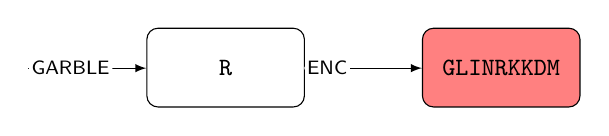
\begin{tikzpicture}
\node[anchor=south west,align=center,package,minimum height=1cm,fill=red!50] (node0) at (7,0.5) {\M{GLINRKKDM}};\node[anchor=south west,align=center,package,minimum height=1cm,fill=white] (node1) at (3.5,0.5) {\M{R}};\draw[-latex,rounded corners]
    (5.5,1) -- node[onarrow] {\O{ENC}} (7,1);
\draw[-latex,rounded corners] (2,1) -- node[onarrow] {\O{GARBLE}} (3.5,1);
\end{tikzpicture}
\hfill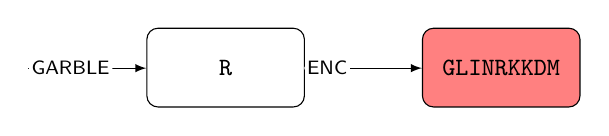
\begin{tikzpicture}
\node[anchor=south west,align=center,package,minimum height=1cm,fill=red!50] (node0) at (7,0.5) {\M{GLINRKKDM}};\node[anchor=south west,align=center,package,minimum height=1cm,fill=white] (node1) at (3.5,0.5) {\M{R}};\draw[-latex,rounded corners]
    (5.5,1) -- node[onarrow] {\O{ENC}} (7,1);
\draw[-latex,rounded corners] (2,1) -- node[onarrow] {\O{GARBLE}} (3.5,1);
\end{tikzpicture}
\hfill\caption{Reduction: RcompGLINRKKDM0 $\approx$ RcompGLINRKKDM1 assuming lin\_rk\_kdm. The sub-graphs corresponding to GLINRKKDM0 and GLINRKKDM1, respectively, are highlighted in red. The remaining graph constitutes the reduction.}\label{figure:reduction:lin_rk_kdm:RcompGLINRKKDM0:RcompGLINRKKDM1}
\end{figure}
\section{Gamehops}
\subsection{Equivalence between RcompGLINRKKDM0 and GSimFreeXORReal}
\subsection{Reduction to lin\_rk\_kdm}
\subsubsection{Game RcompGLINRKKDM0 with Assumption Game GLINRKKDM0 highlighted in red}
\begin{center}
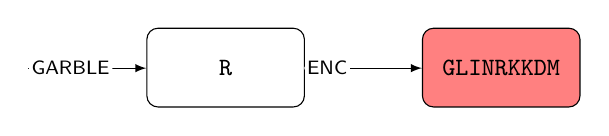
\begin{tikzpicture}
\node[anchor=south west,align=center,package,minimum height=1cm,fill=red!50] (node0) at (7,0.5) {\M{GLINRKKDM}};\node[anchor=south west,align=center,package,minimum height=1cm,fill=white] (node1) at (3.5,0.5) {\M{R}};\draw[-latex,rounded corners]
    (5.5,1) -- node[onarrow] {\O{ENC}} (7,1);
\draw[-latex,rounded corners] (2,1) -- node[onarrow] {\O{GARBLE}} (3.5,1);
\end{tikzpicture}
\end{center}
\subsubsection{Game RcompGLINRKKDM1 with Assumption Game GLINRKKDM1 highlighted  in red}
\begin{center}
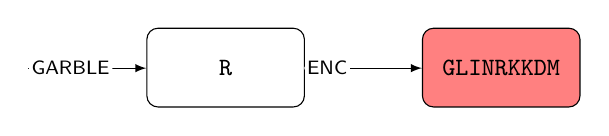
\begin{tikzpicture}
\node[anchor=south west,align=center,package,minimum height=1cm,fill=red!50] (node0) at (7,0.5) {\M{GLINRKKDM}};\node[anchor=south west,align=center,package,minimum height=1cm,fill=white] (node1) at (3.5,0.5) {\M{R}};\draw[-latex,rounded corners]
    (5.5,1) -- node[onarrow] {\O{ENC}} (7,1);
\draw[-latex,rounded corners] (2,1) -- node[onarrow] {\O{GARBLE}} (3.5,1);
\end{tikzpicture}
\end{center}
\end{document}
